% AdjList — Columnar property storage layout
\documentclass[tikz,border=4mm]{standalone}
\usepackage[T1]{fontenc}
\usepackage{lmodern}
% Shared TikZ styles for Flexograph table-layout diagrams.
% Include with % Shared TikZ styles for Flexograph table-layout diagrams.
% Include with % Shared TikZ styles for Flexograph table-layout diagrams.
% Include with \input{schema_styles} in each standalone figure.

\usetikzlibrary{shapes.multipart, arrows.meta, positioning, fit, calc, backgrounds}

% ── Colour palette ──────────────────────────────────────────────────
\definecolor{tblheader}{HTML}{2C3E50}   % dark blue-grey header bar
\definecolor{tblbody}{HTML}{ECF0F1}     % light grey table body
\definecolor{sentbg}{HTML}{D5DBDB}      % sentinel row shading
\definecolor{cgTemporal}{HTML}{AED6F1}  % column group: temporal
\definecolor{cgName}{HTML}{A9DFBF}      % column group: name
\definecolor{cgContact}{HTML}{F9E79F}   % column group: contact
\definecolor{cgLocation}{HTML}{F5CBA7}  % column group: location
\definecolor{cgContent}{HTML}{D2B4DE}   % column group: content
\definecolor{structClr}{HTML}{85929E}   % structural table border
\definecolor{propClr}{HTML}{2980B9}     % property table border
\definecolor{secClr}{HTML}{27AE60}      % secondary table border
\definecolor{arrowClr}{HTML}{7F8C8D}    % relationship arrows

% ── Node styles ─────────────────────────────────────────────────────
\tikzset{
  % Table header bar
  tblhdr/.style={
    rectangle, draw=tblheader, fill=tblheader,
    text=white, font=\sffamily\bfseries\footnotesize,
    minimum width=#1, minimum height=5mm, inner sep=2pt,
    align=center,
  },
  tblhdr/.default=38mm,
  % Table body (single cell / row)
  tblcell/.style={
    rectangle, draw=tblheader!40, fill=tblbody,
    font=\sffamily\scriptsize, minimum width=#1,
    minimum height=4.5mm, inner sep=2pt, align=center,
  },
  tblcell/.default=38mm,
  % Sentinel-row variant
  sentcell/.style={
    tblcell=#1, fill=sentbg,
  },
  sentcell/.default=38mm,
  % Column-group cell (coloured)
  cgcell/.style 2 args={
    tblcell=#1, fill=#2,
  },
  % Key column (narrower, left-aligned)
  keycell/.style={
    tblcell=#1, font=\sffamily\scriptsize\itshape,
  },
  keycell/.default=18mm,
  % Format annotation
  fmtlabel/.style={
    font=\sffamily\tiny\color{tblheader!70}, anchor=north west,
  },
  % Dashed grouping box
  groupbox/.style={
    rectangle, rounded corners=2pt, draw=#1, densely dashed,
    line width=0.6pt, inner sep=3pt,
  },
  groupbox/.default=structClr,
  % Relationship arrow
  relarrow/.style={
    -{Stealth[length=2.5mm]}, arrowClr, line width=0.5pt,
  },
  % Label for relationship
  rellabel/.style={
    font=\sffamily\tiny\color{arrowClr}, midway, fill=white, inner sep=1pt,
  },
}
 in each standalone figure.

\usetikzlibrary{shapes.multipart, arrows.meta, positioning, fit, calc, backgrounds}

% ── Colour palette ──────────────────────────────────────────────────
\definecolor{tblheader}{HTML}{2C3E50}   % dark blue-grey header bar
\definecolor{tblbody}{HTML}{ECF0F1}     % light grey table body
\definecolor{sentbg}{HTML}{D5DBDB}      % sentinel row shading
\definecolor{cgTemporal}{HTML}{AED6F1}  % column group: temporal
\definecolor{cgName}{HTML}{A9DFBF}      % column group: name
\definecolor{cgContact}{HTML}{F9E79F}   % column group: contact
\definecolor{cgLocation}{HTML}{F5CBA7}  % column group: location
\definecolor{cgContent}{HTML}{D2B4DE}   % column group: content
\definecolor{structClr}{HTML}{85929E}   % structural table border
\definecolor{propClr}{HTML}{2980B9}     % property table border
\definecolor{secClr}{HTML}{27AE60}      % secondary table border
\definecolor{arrowClr}{HTML}{7F8C8D}    % relationship arrows

% ── Node styles ─────────────────────────────────────────────────────
\tikzset{
  % Table header bar
  tblhdr/.style={
    rectangle, draw=tblheader, fill=tblheader,
    text=white, font=\sffamily\bfseries\footnotesize,
    minimum width=#1, minimum height=5mm, inner sep=2pt,
    align=center,
  },
  tblhdr/.default=38mm,
  % Table body (single cell / row)
  tblcell/.style={
    rectangle, draw=tblheader!40, fill=tblbody,
    font=\sffamily\scriptsize, minimum width=#1,
    minimum height=4.5mm, inner sep=2pt, align=center,
  },
  tblcell/.default=38mm,
  % Sentinel-row variant
  sentcell/.style={
    tblcell=#1, fill=sentbg,
  },
  sentcell/.default=38mm,
  % Column-group cell (coloured)
  cgcell/.style 2 args={
    tblcell=#1, fill=#2,
  },
  % Key column (narrower, left-aligned)
  keycell/.style={
    tblcell=#1, font=\sffamily\scriptsize\itshape,
  },
  keycell/.default=18mm,
  % Format annotation
  fmtlabel/.style={
    font=\sffamily\tiny\color{tblheader!70}, anchor=north west,
  },
  % Dashed grouping box
  groupbox/.style={
    rectangle, rounded corners=2pt, draw=#1, densely dashed,
    line width=0.6pt, inner sep=3pt,
  },
  groupbox/.default=structClr,
  % Relationship arrow
  relarrow/.style={
    -{Stealth[length=2.5mm]}, arrowClr, line width=0.5pt,
  },
  % Label for relationship
  rellabel/.style={
    font=\sffamily\tiny\color{arrowClr}, midway, fill=white, inner sep=1pt,
  },
}
 in each standalone figure.

\usetikzlibrary{shapes.multipart, arrows.meta, positioning, fit, calc, backgrounds}

% ── Colour palette ──────────────────────────────────────────────────
\definecolor{tblheader}{HTML}{2C3E50}   % dark blue-grey header bar
\definecolor{tblbody}{HTML}{ECF0F1}     % light grey table body
\definecolor{sentbg}{HTML}{D5DBDB}      % sentinel row shading
\definecolor{cgTemporal}{HTML}{AED6F1}  % column group: temporal
\definecolor{cgName}{HTML}{A9DFBF}      % column group: name
\definecolor{cgContact}{HTML}{F9E79F}   % column group: contact
\definecolor{cgLocation}{HTML}{F5CBA7}  % column group: location
\definecolor{cgContent}{HTML}{D2B4DE}   % column group: content
\definecolor{structClr}{HTML}{85929E}   % structural table border
\definecolor{propClr}{HTML}{2980B9}     % property table border
\definecolor{secClr}{HTML}{27AE60}      % secondary table border
\definecolor{arrowClr}{HTML}{7F8C8D}    % relationship arrows

% ── Node styles ─────────────────────────────────────────────────────
\tikzset{
  % Table header bar
  tblhdr/.style={
    rectangle, draw=tblheader, fill=tblheader,
    text=white, font=\sffamily\bfseries\footnotesize,
    minimum width=#1, minimum height=5mm, inner sep=2pt,
    align=center,
  },
  tblhdr/.default=38mm,
  % Table body (single cell / row)
  tblcell/.style={
    rectangle, draw=tblheader!40, fill=tblbody,
    font=\sffamily\scriptsize, minimum width=#1,
    minimum height=4.5mm, inner sep=2pt, align=center,
  },
  tblcell/.default=38mm,
  % Sentinel-row variant
  sentcell/.style={
    tblcell=#1, fill=sentbg,
  },
  sentcell/.default=38mm,
  % Column-group cell (coloured)
  cgcell/.style 2 args={
    tblcell=#1, fill=#2,
  },
  % Key column (narrower, left-aligned)
  keycell/.style={
    tblcell=#1, font=\sffamily\scriptsize\itshape,
  },
  keycell/.default=18mm,
  % Format annotation
  fmtlabel/.style={
    font=\sffamily\tiny\color{tblheader!70}, anchor=north west,
  },
  % Dashed grouping box
  groupbox/.style={
    rectangle, rounded corners=2pt, draw=#1, densely dashed,
    line width=0.6pt, inner sep=3pt,
  },
  groupbox/.default=structClr,
  % Relationship arrow
  relarrow/.style={
    -{Stealth[length=2.5mm]}, arrowClr, line width=0.5pt,
  },
  % Label for relationship
  rellabel/.style={
    font=\sffamily\tiny\color{arrowClr}, midway, fill=white, inner sep=1pt,
  },
}


\begin{document}
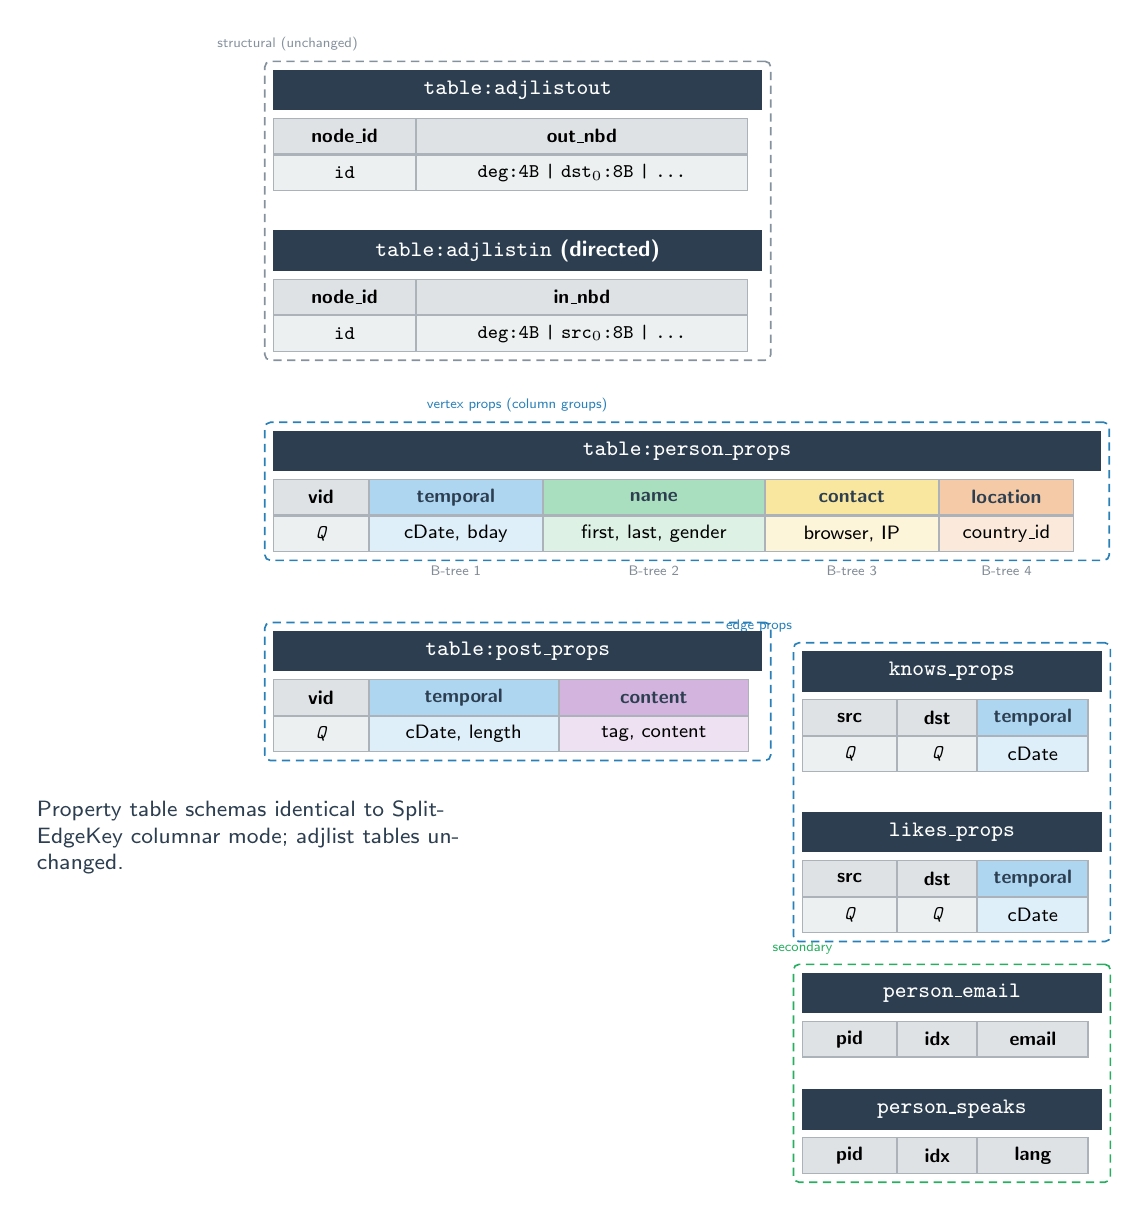
\begin{tikzpicture}[node distance=0mm]

% ════════════════════════════════════════════════════════════════════
%  STRUCTURAL: adjlistout + adjlistin  (unchanged from embedded)
% ════════════════════════════════════════════════════════════════════
\node[tblhdr=62mm] (aout-hdr) {\texttt{table:adjlistout}};

\node[tblcell=18mm, below=1mm of aout-hdr.south west, anchor=north west,
      fill=tblheader!15, font=\sffamily\scriptsize\bfseries] (ao-ch-k)
  {node\_id};
\node[tblcell=42mm, right=0mm of ao-ch-k,
      fill=tblheader!15, font=\sffamily\scriptsize\bfseries] (ao-ch-v)
  {out\_nbd};

\node[tblcell=18mm, below=0mm of ao-ch-k] (ao-r1-k) {\texttt{id}};
\node[tblcell=42mm, right=0mm of ao-r1-k] (ao-r1-v)
  {\texttt{deg:4B\;|\;dst$_0$:8B\;|\;\ldots}};

\node[tblhdr=62mm, below=5mm of ao-r1-k.south west, anchor=north west]
  (ain-hdr) {\texttt{table:adjlistin} {\footnotesize(directed)}};

\node[tblcell=18mm, below=1mm of ain-hdr.south west, anchor=north west,
      fill=tblheader!15, font=\sffamily\scriptsize\bfseries] (ai-ch-k) {node\_id};
\node[tblcell=42mm, right=0mm of ai-ch-k,
      fill=tblheader!15, font=\sffamily\scriptsize\bfseries] (ai-ch-v) {in\_nbd};
\node[tblcell=18mm, below=0mm of ai-ch-k] (ai-r1-k) {\texttt{id}};
\node[tblcell=42mm, right=0mm of ai-r1-k] (ai-r1-v)
  {\texttt{deg:4B\;|\;src$_0$:8B\;|\;\ldots}};

% ════════════════════════════════════════════════════════════════════
%  PROPERTY TABLES: person_props (4 column groups)
% ════════════════════════════════════════════════════════════════════
\node[tblhdr=105mm, below=10mm of ai-r1-k.south west, anchor=north west]
  (pp-hdr) {\texttt{table:person\_props}};

\node[cgcell={12mm}{white}, below=1mm of pp-hdr.south west,
      anchor=north west,
      fill=tblheader!15, font=\sffamily\scriptsize\bfseries] (pp-k) {vid};
\node[cgcell={22mm}{cgTemporal},  right=0mm of pp-k,
      font=\sffamily\scriptsize\bfseries] (pp-cg1)
  {\textcolor{tblheader}{temporal}};
\node[cgcell={28mm}{cgName},      right=0mm of pp-cg1,
      font=\sffamily\scriptsize\bfseries] (pp-cg2)
  {\textcolor{tblheader}{name}};
\node[cgcell={22mm}{cgContact},   right=0mm of pp-cg2,
      font=\sffamily\scriptsize\bfseries] (pp-cg3)
  {\textcolor{tblheader}{contact}};
\node[cgcell={17mm}{cgLocation},  right=0mm of pp-cg3,
      font=\sffamily\scriptsize\bfseries] (pp-cg4)
  {\textcolor{tblheader}{location}};

\node[keycell=12mm, below=0mm of pp-k] (pp-fk) {\texttt{Q}};
\node[cgcell={22mm}{cgTemporal!40}, right=0mm of pp-fk] (pp-f1)
  {cDate, bday};
\node[cgcell={28mm}{cgName!40},     right=0mm of pp-f1] (pp-f2)
  {first, last, gender};
\node[cgcell={22mm}{cgContact!40},  right=0mm of pp-f2] (pp-f3)
  {browser, IP};
\node[cgcell={17mm}{cgLocation!40}, right=0mm of pp-f3] (pp-f4)
  {country\_id};

\node[font=\sffamily\tiny, text=tblheader!60, below=0.5mm of pp-f1]
  {B-tree 1};
\node[font=\sffamily\tiny, text=tblheader!60, below=0.5mm of pp-f2]
  {B-tree 2};
\node[font=\sffamily\tiny, text=tblheader!60, below=0.5mm of pp-f3]
  {B-tree 3};
\node[font=\sffamily\tiny, text=tblheader!60, below=0.5mm of pp-f4]
  {B-tree 4};

% ── post_props ──────────────────────────────────────────────────
\node[tblhdr=62mm, below=10mm of pp-fk.south west, anchor=north west]
  (post-hdr) {\texttt{table:post\_props}};

\node[cgcell={12mm}{white}, below=1mm of post-hdr.south west,
      anchor=north west,
      fill=tblheader!15, font=\sffamily\scriptsize\bfseries] (po-k) {vid};
\node[cgcell={24mm}{cgTemporal}, right=0mm of po-k,
      font=\sffamily\scriptsize\bfseries] (po-cg1)
  {\textcolor{tblheader}{temporal}};
\node[cgcell={24mm}{cgContent}, right=0mm of po-cg1,
      font=\sffamily\scriptsize\bfseries] (po-cg2)
  {\textcolor{tblheader}{content}};

\node[keycell=12mm, below=0mm of po-k] (po-fk) {\texttt{Q}};
\node[cgcell={24mm}{cgTemporal!40}, right=0mm of po-fk] (po-f1)
  {cDate, length};
\node[cgcell={24mm}{cgContent!40}, right=0mm of po-f1] (po-f2)
  {tag, content};

% ── knows_props + likes_props ───────────────────────────────────
\coordinate (edge-anchor) at ($(post-hdr.east) + (5mm, 0)$);

\node[tblhdr=38mm, anchor=north west] at (edge-anchor) (kp-hdr)
  {\texttt{knows\_props}};
\node[cgcell={12mm}{white}, below=1mm of kp-hdr.south west,
      anchor=north west,
      fill=tblheader!15, font=\sffamily\scriptsize\bfseries] (kp-k1) {src};
\node[cgcell={10mm}{white}, right=0mm of kp-k1,
      fill=tblheader!15, font=\sffamily\scriptsize\bfseries] (kp-k2) {dst};
\node[cgcell={14mm}{cgTemporal}, right=0mm of kp-k2,
      font=\sffamily\scriptsize\bfseries] (kp-cg)
  {\textcolor{tblheader}{temporal}};
\node[keycell=12mm, below=0mm of kp-k1] (kp-fk1) {\texttt{Q}};
\node[keycell=10mm, right=0mm of kp-fk1] (kp-fk2) {\texttt{Q}};
\node[cgcell={14mm}{cgTemporal!40}, right=0mm of kp-fk2] (kp-f1) {cDate};

\node[tblhdr=38mm, below=5mm of kp-fk1.south west, anchor=north west]
  (lp-hdr) {\texttt{likes\_props}};
\node[cgcell={12mm}{white}, below=1mm of lp-hdr.south west,
      anchor=north west,
      fill=tblheader!15, font=\sffamily\scriptsize\bfseries] (lp-k1) {src};
\node[cgcell={10mm}{white}, right=0mm of lp-k1,
      fill=tblheader!15, font=\sffamily\scriptsize\bfseries] (lp-k2) {dst};
\node[cgcell={14mm}{cgTemporal}, right=0mm of lp-k2,
      font=\sffamily\scriptsize\bfseries] (lp-cg)
  {\textcolor{tblheader}{temporal}};
\node[keycell=12mm, below=0mm of lp-k1] (lp-fk1) {\texttt{Q}};
\node[keycell=10mm, right=0mm of lp-fk1] (lp-fk2) {\texttt{Q}};
\node[cgcell={14mm}{cgTemporal!40}, right=0mm of lp-fk2] (lp-f1) {cDate};

% ── Secondary: person_email, person_speaks ──────────────────────
\node[tblhdr=38mm, below=5mm of lp-fk1.south west, anchor=north west]
  (pe-hdr) {\texttt{person\_email}};
\node[tblcell=12mm, below=1mm of pe-hdr.south west, anchor=north west,
      fill=tblheader!15, font=\sffamily\scriptsize\bfseries] (pe-k1) {pid};
\node[tblcell=10mm, right=0mm of pe-k1,
      fill=tblheader!15, font=\sffamily\scriptsize\bfseries] (pe-k2) {idx};
\node[tblcell=14mm, right=0mm of pe-k2,
      fill=tblheader!15, font=\sffamily\scriptsize\bfseries] (pe-v) {email};

\node[tblhdr=38mm, below=4mm of pe-k1.south west, anchor=north west]
  (ps-hdr) {\texttt{person\_speaks}};
\node[tblcell=12mm, below=1mm of ps-hdr.south west, anchor=north west,
      fill=tblheader!15, font=\sffamily\scriptsize\bfseries] (ps-k1) {pid};
\node[tblcell=10mm, right=0mm of ps-k1,
      fill=tblheader!15, font=\sffamily\scriptsize\bfseries] (ps-k2) {idx};
\node[tblcell=14mm, right=0mm of ps-k2,
      fill=tblheader!15, font=\sffamily\scriptsize\bfseries] (ps-v) {lang};

% ── Grouping boxes ──────────────────────────────────────────────
\begin{pgfonlayer}{background}
  \node[groupbox=structClr, fit=(aout-hdr)(ai-r1-v),
        label={[font=\sffamily\tiny,
        text=structClr]above left:structural (unchanged)}] {};
  \node[groupbox=propClr, fit=(pp-hdr)(pp-f4),
        label={[font=\sffamily\tiny,
        text=propClr]above left:vertex props (column groups)}] {};
  \node[groupbox=propClr, fit=(post-hdr)(po-f2)] {};
  \node[groupbox=propClr, fit=(kp-hdr)(lp-f1),
        label={[font=\sffamily\tiny,
        text=propClr]above left:edge props}] {};
  \node[groupbox=secClr, fit=(pe-hdr)(ps-v),
        label={[font=\sffamily\tiny,
        text=secClr]above left:secondary}] {};
\end{pgfonlayer}

% ── Note ────────────────────────────────────────────────────────
\node[font=\sffamily\footnotesize, text=tblheader, anchor=north west,
      below=5mm of po-fk.south west, text width=60mm]
  {Property table schemas identical to SplitEdgeKey columnar mode;
   adjlist tables unchanged.};

\end{tikzpicture}
\end{document}
